% Template as of 22.04.2021 error free
%%%%%%%%%%%%%%%%%%%%%%%%%%%%%%%%%%%%%%%%%%%
\documentclass[a4paper,5p,review]{elsarticle}
%\documentclass[final,5p,times,twocolumn]{elsarticle}

\usepackage{lineno}
\usepackage{easylist}
\usepackage{amssymb}
\usepackage{amsmath}
\usepackage{subcaption}
\usepackage[breaklinks]{hyperref}
\usepackage{url}
\usepackage{textcomp}
\usepackage{verbatim}
\usepackage[ruled,vlined]{algorithm2e}
\usepackage{ulem}
%\usepackage[ampersand]{easylist}
\setcounter{tocdepth}{3}
\usepackage{graphicx}
\usepackage{pgfplots}
\usepackage{listings} 
\pgfplotsset{compat=1.14}
\pgfplotsset{compat=newest}
\pgfplotsset{plot coordinates/math parser=false}
\usepackage{tikzscale}
\usetikzlibrary{matrix,chains,positioning,decorations.pathreplacing,arrows}
\usepackage{tikz-qtree,tikz-qtree-compat}
\usetikzlibrary{calc}
\modulolinenumbers[5]

\journal{Journal of \LaTeX\ Templates}

%%%%%%%%%%%%%%%%%%%%%%%
%% Elsevier bibliography styles
%%%%%%%%%%%%%%%%%%%%%%%
%% To change the style, put a % in front of the second line of the current style and
%% remove the % from the second line of the style you would like to use.
%%%%%%%%%%%%%%%%%%%%%%%

%% Numbered
%\bibliographystyle{model1-num-names}

%% Numbered without titles
%\bibliographystyle{model1a-num-names}

%% Harvard
%\bibliographystyle{model2-names.bst}\biboptions{authoryear}

%% Vancouver numbered
%\usepackage{numcompress}\bibliographystyle{model3-num-names}

%% Vancouver name/year
%\usepackage{numcompress}\bibliographystyle{model4-names}\biboptions{authoryear}

%% APA style
%\bibliographystyle{model5-names}\biboptions{authoryear}

%% AMA style
%\usepackage{numcompress}\bibliographystyle{model6-num-names}

\pdfstringdefDisableCommands{%
  \def\corref#1{}%
}

%% `Elsevier LaTeX' style
\bibliographystyle{elsarticle-num}
%%%%%%%%%%%%%%%%%%%%%%%

\begin{document}

\begin{frontmatter}

\title{Crisp, Short, Clear, Concise Title of the Paper}

%% or include affiliations in footnotes:
\author[TUB]{Theodore Evans\corref{mycorrespondingauthor}}
\cortext[mycorrespondingauthor]{Corresponding author}
\ead{theodor.evans@dai-labor.de}
\author[TUB]{Christian Geissler}
\author[TUB]{Carl Ogre Retzlaff}
\author[CAR]{Norman Zerbe}
\author[xxx]{Erika Musterfrau}
\author[xxx]{Max Mustermann}
\author[MUG]{Markus Plass}
\author[MUG]{Heimo Mueller}
\author[MUG,amii]{Andreas Holzinger }


\address[TUB]{DAI, Technical University Berlin, Germany}
\address[MUG]{Medical University Graz, Austria}
\address[amii]{Alberta Machine Intelligence Institute, Canada}
\address[xxx]{Lab Name, University Name, Address}

\begin{abstract} 
What was already known on the topic to the international research community ?
%This must be shortened still !! 
% NOTE- PLACEHOLDER TEXT ONLY. This text was pulled directly from the call for papers on Elsevier website. Should be completely rewritten, not just adapted
The spread of the use of artificial intelligence techniques is now ubiquitous and unstoppable. It brings many opportunities and helps solve old problems. However, by its very nature, the use of AI also brings many risks and new problems that must be addressed to avoid jeopardizing effective evolution. The emerging field of eXplainable AI (XAI) is helping to find answers to these problems and put people more at the center.
While from a research perspective, discussions of XAI date back several decades and were reinvigorated by the DARPA initiative, the concept emerged with renewed vigor in late 2019 when Google announced a new XAI toolset for developers after announcing its "AI-first" strategy in 2017. This is because many of today's machine and deep learning applications do not allow us to fully understand how they work or the logic behind them, which is referred to as a "black box." The high complexity makes many successful machine learning models difficult or impossible to understand. This characteristic is considered one of the biggest problems in the application of AI techniques; it makes machine decisions non-transparent and often incomprehensible even to experts or developers. Explainable AI systems can explain the logic of decisions, characterize the strengths and weaknesses of decision making, and provide insights into their future behavior.
What this paper contributes to the international research community ?

This paper describes, analyzes  ...

The novelty is, the results show, the paper demonstrates ...

The benefit is, it indicates that ...



%The spread of the use of artificial intelligence techniques is now pervasive and unstoppable. However, it brings with its opportunities but also risks and problems that must be addressed in order not to compromise an effective evolution. The eXplainable AI (XAI) is one of the answers to these problems to bring humans closer to machines. While from a research perspective the discussions on XAI date back a few decades, the concept emerged with renewed vigour at the end of 2019 when Google, after announcing its "AI-first" strategy in 2017, recently announced a new XAI toolset for developers. Nowadays many of the machine and deep learning applications do not allow you to understand how they work entirely or the logic behind them for effect called "BlackBox", according to which machine learning models are mostly black boxes. This feature is considered one of the biggest problems in the application of AI techniques; it makes machine decisions not transparent and often incomprehensible even to the eyes of experts or developers themselves. Explainable AI systems can explain the logic of decisions, characterize the strengths and weaknesses of decision making, and provide insights into their future behaviour.
\end{abstract}

\begin{keyword}
Explainable AI, interpretable Machine Learning, interactive Machine Learning, aggregation functions, ordinal sums, Glass--box approach, transparency 
\end{keyword}

\end{frontmatter}
\linenumbers

%%%%%%%%%%%%%%%%%%%%%%%%%%%%%%%%%%%%%%%%%%%%%%%%%%%%%%%%%%%%%%%%%%%%%%%%%%%%%%%%%%%%%%%%%%%%%%%%%%%%%%%%%%%%%%%%%%%%%%%%%%%%%%%%%%%%%%%%
% OVERVIEW

% Motivation
% - Explainability as cross-disciplinary, embedded concept
% - Limitations of focusing on either algorithmic or UX aspects alone
% - Need for deeper, cross-disciplinary study of explainability requirements in a specific context

% Outcome
% - Exploratory case study 
% - Investigating the understandability, informativeness and value to user for
% - n 'explanation classes', with presentation modalities chosen to be appropriate
% - For a representative Ki-67 AI solution, with model outputs of generated annotations and overall nuclear positivity
% - analysed with respect to users' usage / familiarity with AI solutions/ ML in general

% Future work
% - Technical implementations for classes of explanation that are understandable, provide insight and value, but are currently not represented in the SOA

%%%%%%%%%%%%%%%%%%%%%%%%%%%%%%%%%%%%%%%%%%%%%%%%%%%%%%%%%%%%%%%%%%%%%%%%%%%%%%%%%%%%%%%%%%%%%%%%%%%%%%%%%%%%%%%%%%%%%%%%%%%%%%%%%%%%%%%%

\section*{\textbf{Highlights}}

\begin{itemize}
    \item This paper describes, analyzes, 
    \item The novelty is, the results show, the paper demonstrates
    \item The benefit is, it indicates that, 
\end{itemize}
%First paper that evaluates XAI-Approaches in the Pathology domain!!!

\section{Introduction}
\label{sec:introduction}

Pathology is poised at the brink of an AI renaissance. For one hundred and fifty years, the analysis of tissue has taken place primarily through the lens of a microscope. In the last decade, the growing proliferation of digitized diagnostic workflows has intersected with the explosive growth of successful machine learning (ML) capabilities~\cite{Pantanowitz:2010:DigitalPathology,PantanowitzEtAl:2021:AIPatho}, promising improved patient outcomes and reduced clinician workloads through the automation of repetitive tasks~\cite{das2020computer}. These advances in computational methods for pathology, combined with increasing availability of patient *omics (genomics, proteomics, metabolomics, etc.) and electronic health record (EHR) data, open the door to a new era of AI/ML-assisted personalized medicine~\cite{acs2020artificial,holzinger_artificial_2020}.

However, the lack of human-interpretability inherent to many machine learning models remains a barrier to their acceptance and approval for clinical application~\cite{cui2021artificial}. Without a clear understanding of the factors important to the algorithmic decision-making process, including potential limitations and sources of bias, medical practitioners can not use these results as the basis for potentially life-altering clinical decisions. This requirement is not only an ethical accountability issue, but has also been identified as a critical component in the evolving landscape defining regulations, norms, and standards for the safe use of AI/ML-based software as a medical device (SaMD)~\cite{EU_White, ISO_IEC_TR_24028}. 

Recognising this need, the body of research on explainable AI (xAI) for medicine has grown exponentially~\cite{tjoa_survey_2020,poceviciute_survey_2020}. While the exact definition is a matter of some debate, we refer to explainable AI as that whose internal workings, if not directly interpretable, can be communicated to the user in an adaptive, understandable way. This concept of explainability is multifaceted; not only requiring communicable insights to be distilled from the inherent complexity of so-called ``black-box'' models, but also in knowing what, and in what modality, information should be presented to a given user or stakeholder~\cite{HolzingerEtAl:2020:QualityOfExplanations,zednik2019solving}.

Despite the multifaceted nature of such questions, the current research landscape exhibits a lack of dedicated interdisciplinary work to this effect~\cite{antoniadi2021current}. To date, only a handful of studies have attempted to bridge the gap between technical implementation and user experience of explainability in medical AI~\cite{liao2020questioning,cai2019hello,wang_designing_2019}. While such human-centric studies have been identified as critical to the development of safe and effective xAI systems~\cite{doshi2017towards, regitnig_expectations_2020, antoniadi2021current}, no study has yet been conducted to evaluate the interaction of real pathologists with task-specific explanation generation techniques.

% While there exist valuable efforts to collect and categorise the broad range of algorithmic approaches to xAI -- both generally \cite{arrieta2020explainable} and as specifically applied to medicine \cite{tjoa_survey_2020, deshpande2021brief} and in particular, digital pathology~\cite{poceviciute_survey_2020}, 

% The involvement of the target audience is especially relevant in the field of explainable AI, as the quality of explanations is a function of the needs and propensities of the users within the context of a particular task and data modality -- in this case, a specific diagnostic workflow. That is to say, the evaluation of xAI approaches in other fields does not necessarily transfer to the field of digital pathology.

To address this need, we conducted a mixed-methods study, assessing the interpretation and usability of a set of examples representing the state of the art in explanation-generating methods for image analysis, as applied to a common AI-assisted task in digital pathology. This study aims to answer the following questions:

\researchquestions

As well as providing valuable insights for the development of safer and more effective xAI solutions in pathology, this research serves as a template for further user- and application-grounded studies within medicine as well as further afield.

\section{Background and Related Work}

There is general consensus in the scientific community that the broad field of AI has great potential to support a variety of workflows in practically every sub-domain of medicine~\cite{hamet2017artificial}, but particularly in medical imaging fields such as radiology and pathology~\cite{WulczynEtAl:2021:AImed-example}.

This trend has been sparked by the tremendous success in statistical machine learning; in particular, the success of the sub-family of deep learning driven by the availability of enhanced computing resources and increasing volumes of machine-readable data~\cite{LeCunBengioHinton:2015:DeepLearningNature}. It promises great positive impact on diagnosticians by improving workflows, reducing errors~\cite{Topol:2019:NatureMedicine} and building a fundamental basis for future precision medicine solutions. However, the best performing machine learning methods are often so high-dimensional and complex that results are difficult, if not impossible, for a human expert to understand. Such methods, of which deep neural networks represent the most prominent example, are colloquially referred to as ``black-box'' models~\cite{Castelvecchi:2016:OpenBlack}.

One solution to this problem could be avoidance of black-box approaches in favour of those that are inherently interpretable, as \citet{Rudin:2019:interpretable} recommends. While this may be feasible for certain classes of problem, for complex tasks and those with high dimensional input, as is the case for many image analysis tasks in pathology, performance of interpretable models is generally far outclassed by black-box approaches~\cite{arrieta2020explainable, Holzinger:2020:explainable}.

The goal of xAI research is to resolve this dilemma by enabling AI systems to make intelligible, to a human stakeholder, the reasons for which a black-box model produced a particular result. Rapid growth of explainability research for medical AI is driven not only by evolving ethical~\cite{MuellerEtAl:2021:TenCommandments} and regulatory~\cite{Schneeberger:2020:legalAI} concerns, but also as a means to foster trust and acceptance of AI solutions by their target users~\cite{GuidottiPedreschi:2019:Survey, ProsperiEtAl:2020:CausalHealth, Ferrario:trustmedicalai, gaube:trustmedicalai:2021, kastner2021relation}.

As well as a solution to this growing challenge, xAI is identified as a key component of hybrid intelligence systems, in which human and AI work together collaboratively ~\cite{hemmer2021human}. In the near future, such systems may allow diagnosticians to dynamically interact with an AI system through queries and counterfactuals~\cite{HolzingerEtAl:2021:GraphFusion}, or for AI systems to improve their performance by actively bringing the human into the machine learning loop~\cite{Holzinger:2020:explainable}.

% In 2020, the European Commission published a White Paper on the safety and liability implications of AI, which suggests mandatory re-traceability, interpretability, explainability (in a juridical sense) of AI systems in critical domains \cite{Schneeberger:2020:legalAI}. While medical decision support is not identified from the outset as a ``high-risk" AI application area in the proposed EU Artificial Intelligence Act of 2021, this act would nonetheless set a precedent for legally mandated implementation of transparency and explainability in AI systems~\cite{EU:2021:52021PC0206}.

% -> HCI section

%However, even the best human experts sometimes cannot explain something, but rather construct mental models intuitively of the problem and consult these models to select the best possible solution from a set of options \cite{HudecEtAl-2021-Interpretable}.

% A good example is a very recent work where the findings indicate that the primary value of human-in-the-loop corrections is to address significant weaknesses of a digital image analysis application, rather than fine-tuning the digital image analysis quantification \cite{BodenLundstrom:2021:HumanPatho}.

% If such approaches are to be introduced successfully into the workflow of digital pathology \cite{Kargl-et-al:2020:PathoWorkflows}, such approaches need new kinds of Human-AI interfaces. 

% This is important because in the medical field, it is crucial that domain knowledge be brought in to infer causal effects. In fact, according to the current state of research, this domain knowledge, which is ignored in classical statistical machine learning, is crucial \cite{Pearl:2019:CACM,ProsperiEtAl:2020:CausalHealth}. 

\subsection{Cross-disciplinary views on xAI}

\citet{miller2019explanation} places xAI research at the intersection between AI, social science and human-computer interface (HCI) research. Accordingly, there is a body of research from these domains that either deal directly with~\cite{abdul2020cogam, holzinger2013human}, or are directly applicable to~\cite{nielsen2005ten}, topics of xAI development.

Applications of social and cognitive science to the field of xAI~\cite{de2017people, miller2019explanation, lipton2018mythos, jussupow2021augmenting} highlight the non-idealised way in which human beings make decisions, and accordingly, interact with decision-making systems. Notably, \citet{wang_designing_2019} build upon this theoretical work~\cite{hoffman2017explainingpart1,hoffman2017explainingpart2, klein2018explainingpart3, hoffman2018explainingpart4} to propose concrete guidelines for the design of user-centric xAI that mitigates (rather than exacerbates) sources of bias and error in human reasoning.

While metrics and evaluation strategies for explanation-generating techniques themselves have been proposed~\cite{doshi2017towards, HolzingerEtAl:2019:Wiley-Paper, HolzingerEtAl:2020:QualityOfExplanations}, studies of these in user- and application-grounded contexts are in their infancy. Those studies having been conducted deal primarily with evaluating the explainability requirements of users with respect to a novel AI system~\cite{liao2020questioning, cai2019hello}. 

% TODO: Add Kargl paper here

Our study extends this valuable prior work by evaluating the interactions of users with explainability techniques themselves, where these are potentially previously unseen by users. Given the sensitivity of such methods to the effects of bias, as identified in the literature, this represents an important contribution to the xAI research landscape.

% % interactivity
% \citet{abdul2020cogam} recognise the importance of managing cognitive load in xAI systems, and propose an approach to dynamically adapting the complexity of explanations to the needs of the user.
% % \cite{wang_designing_2019}
% % This capacity for an AI system to effectively communicate decision factors is considered of particular importance to the development of future human-AI interfaces. These range from interactive systems that dynamically provide contextual information, responding to questions and counterfactuals from the user~\cite{HolzingerEtAl:2021:GraphFusion}, to hybrid human-machine systems that are capable of outperforming either party in isolation~\cite{Holzinger:2016:iML}.

% Work has been done to define The ability of a human stakeholder to effectively infer the causal factors behind predictions is identified as a critical component of effective medical xAI~\cite{HolzingerEtAl:2019:Wiley-Paper, HolzingerEtAl:2020:QualityOfExplanations}. \citet{} define \textit{causability} as a metric measuring the extent to which an explanation imparts a user with causal understanding of an AI system in a given context.

\subsection{Classes of Explanation-Generating Methods}
\label{sec:related:classes}

Given their context-sensitive nature, defining a single, comprehensive taxonomy of xAI methods is -- and will likely remain -- an open question. However, valuable efforts have been made to survey the algorithmic state of the art~\cite{tjoa_survey_2020, deshpande2021}, with various schemata having been been developed to categorise these approaches~\cite{arrieta2020explainable}.

Dealing specifically with those approaches directly applicable to the typical tasks and model architectures of digital pathology, \citet{poceviciute_survey_2020} comprehensively collects and categorises the state of the art in xAI methods along three axes: the type of information to be conveyed, the way in which results are represented to the user, and the technical approach employed in their generation. A similar, HCI-oriented taxonomy is presented by \citet{liao2020questioning}. 

The presentation modalities of image-applicable explanation generation methods can be broadly categorised into four classes, ordered by prevalence: Saliency maps, Concept attribution, Prototypes and Counterfactuals~\cite{bodria_benchmarking_2021}.

\textbf{Saliency maps} aim to explain individual predictions through visualisations on the input \cite{MorchEtAl:1995:Saliency}. This is generally manifested as an overlay on the input image, indicating the \textit{saliency} per pixel or image region to the model in question. Depending on implementation, saliency may represent a measure of intrinsic informational content~\cite{KadirBrady:2001:Saliency}, or the estimated relevance to a particular model outcome or feature~\cite{SimonyanVedaldiZisserman:2013:DeepInside, springenberg2014striving, yosinski2015deepvisualization, LapuschkinEtAl:2016:LRP, selvaraju2017grad, ribeiro2018anchors}.

\textbf{Concept attribution}-based approaches aim to explain individual predictions or model inner workings with respect to a set of high-level concepts, either by their presence in a model's learned representation ~\cite{GrazianiHenning:2020:ConceptAttribution} or their importance to a particular model outcome~\cite{kim2018interpretability}. These high-level concepts may be represented as synthetic visualisations~\cite{erhan2009visualizing, yosinski2015deepvisualization}, or in terms of domain-specific natural language~\cite{GrazianiHenning:2020:ConceptAttribution, kim2018interpretability} 

\textbf{Prototypes} are explanations of model inner workings through representations of the archetypal instance of a particular class, feature or model outcome. These prototypical examples may be synthetic visualisations~\cite{li2018deep} or real examples~\cite{kim2016examples}.

\textbf{Counterfactuals} aim to explain a model outcome by presenting one or more "what if..." scenarios -- examples of similar inputs that would lead to a different model outcomes~\cite{ginsberg1986counterfactuals}. While these counterfactual examples are mainly generated as synthetic visualisations~\cite{seah2019chest, poceviciute_survey_2020, liu2019generative}, these may be supplemented by examples from real data~\cite{gulshad2021counterfactual}.

While measures that indicate the trustworthiness of model outcomes without directly relating the causal factors underlying them may not be considered explanations \textit{per se}, there is a precedent for bringing these under the umbrella of xAI~\cite{poceviciute_survey_2020, lin2019explanations}.

\textbf{Trust Scores} refer to generated measures indicating confidence, certainty or otherwise trustworthiness of a model and its outcomes, in particular, those that supplement or replace a model's own self-assessed, and therefore potentially biased, confidence~\cite{jiang2018trust, wang2021ai}. These may be derived from the trained model itself~\cite{tagasovska2019single}, or from the output of an independent model~\cite{jiang2018trust} or ensemble of models~\cite{pearce2018high}.

It should be noted that these classes are neither comprehensive nor mutually exclusive, with many approaches combining features from different classes~\cite{kim2016examples,liu2019generative}. Recent work surveying the literature challenges the boundaries between some of these categories outright~\cite{zhang2021survey}. While the authors are inclined to agree with this assessment, the above-described classes nevertheless provide a useful basis on which to compare the interpretation and usability of explanation modalities by their target audience.


% %Backup-text for EMPAIA by Christian:
% Within the project EMPAIA \cite{empaia-website} that deals with lowering the hurdles of translating AI application into clinical practice, the question of how exactly xAI can help with making AI applications safe and reliable to use in routine practice plays a crucial role. The following Ki-67 use case was selected from the available solutions as a first step to investigate xAI methods for a specific exemplary use case. The choice was discussed and made in a project-related validation committee, an open panel of medical and AI experts.

% The goal of all of these efforts is a very central one: to promote and to ensure trust in AI\cite{LakkarajuLeskovec:2019:trust}. Any use of AI in digital pathology will not work if there is a lack of trust. And that is the problem, because in a "black box" application, trust would mean blindly relying on a medical AI \cite{Ferrario:trustmedicalai}, \cite{gaube:trustmedicalai:2021} without being able to re-trace, check and understand the results. Consequently, trust is inherently connected to and builds on both legal aspects\cite{Schneeberger:2020:legalAI} and ethical principles\cite{MuellerEtAl:2021:TenCommandments}. 

% In the very tentative developing relationship between humans and AI, trust is the only mechanism that actually influences clinicians' use and adoption of AI \cite{asan:trustmedicalai:2020}. 

% This is because trust is a profoundly human psychological mechanism for dealing with uncertainty between what is known and what is unknown \cite{Corazzini:1977:trust},\cite{Simpson:2007:trust}. Some recent studies show that even consumers are reluctant to use health services provided by AI - and prefer the "humanity" of decisions \cite{Longoni:2019:resistance}. Furthermore, trust is very tightly connected with acceptance \cite{Venkatesh:2003:acceptance}.

% In digital pathology, however, this is precisely the problem because acceptance of unfamiliar technology is very strongly linked to technology affinity in general and to prior technical experience, a factor known as previous exposure to technology (PET) \cite{Holzinger:2011:acceptance}. Generally, the end users in the medical domain are reluctant to utilize healthcare provided by AI in real and hypothetical choices, separate and joint evaluations.


% Proposal of a paragraph (Tomasz' older contribution) - to be put here or in \subsection{Relationship to Human-Computer Interaction}, if accepted

%  Tools designed to support human-computer interaction by means of involving the sense of sight, 
%  especially in a digital environment, allow to morphometry and visualization 
%  of medical multimodal and dynamical data \cite{soltysinski2007HCI}. The applications of 
%  medical noisy data segmentation for the purpose of presentation and diagnostics can be 
%  directly transfered into digital pathology supported by AI. Such methods apply to 
%  digitized tissue data obtained from label-free optical imaging \cite{Golniketal2008micropolar}.
%  Moreover, the attention of the investigator can be quantified through multimodal scanning 
%  of their behavioral and mental activity \cite{Soltysinski2006EEG}. 

%Norman, Tomasz

%Ki-67 Use case description
% Rasmus & Norman

\section{State of the art}
\label{sec:SOA}

\cite{holzinger_artificial_2020} and \cite{piccialli_survey_2021} (guest editor paper) state of the art on AI applications in medicine and growing prevalence of AI solutions in medicine

\cite{piccialli_artificial_2021} (two guest editors on this one) and \cite{HolzingerEtAl:2021:GraphFusion} for the future direction of AI approaches in medicine, combining data over time and from multiple modalities, dramatically increasing the need for explainability/causability, as the total model input cannot be simply inspected by a user (as is currently the case)

\cite{tjoa_survey_2020} for state of the art in XAI solutions for medicine, highlights the shortcomings of an algorithm-focused research landscape in addressing explainability needs of users in practice

\cite{poceviciute_survey_2020} for the most pathology-specific analysis of XAI approaches, basis for building the explanation classes

\cite{bodria_benchmarking_2021} (could also be introduced in case study design) introduces explanation classes and benchmarks for the evaluation of XAI approaches

Also to include: 
\begin{itemize}
\item current regulatory landscape wrt. explainability for AI solutions
\item state of the art for (selected) technical implementations of explainability?
\end{itemize}


ui subsection:
show old ui rules
keep human in control as per eu regulation
ai is not really integrated into old hci, need a new ai ui connection
\cite{tosun_histomapr_2020} XAI UI for pathology
% Tomasz, Andreas, Norman, Christian, Theodore, Carl

%User Interface SotA for medical applications

\section{Case study design}
\label{sec:CaseStudyDesign}

\cite{chakraborti_emerging_2020} identifies the need for understanding the 'personae' of stakeholders

\subsection{Selection of AI solutions}

Ki-67 app(s) selected based on xyz, 
Possible criteria:

\begin{itemize}
    \item CE-IVD approved for clinical use
    \item black-box algorithm (i.e. DL)
    \item results not easily verifiable by clinician with cursory visual inspection
\end{itemize}

% Candidates:
% - Visiopharm Ki-67 app (https://visiopharm.com/app-center/app/ki-67-app-breast-cancer/, demo: https://www.labroots.com/ms/webinar/standardization-clinical-digital-pathology-ki-67)
% - Roche VENTANA Companion Algorithm Ki-67 (30-9) (https://diagnostics.roche.com/no/en/products/instruments/ventana-companion-algorithm-image-analysis-software.html), also has FDA 510(k) clearance
% - MindPeak BreastIHC (https://www.mindpeak.ai/products/mindpeak-breastihc) CE-IVD clearance pending

\subsection{Selection of stakeholders}

User personae 1-3 based on xyz. \cite{poceviciute_survey_2020} Ongoing work by Graz? @Andreas
Stakeholders selected from EMPAIA Gremien members

\subsection{Research questions}

Research questions based on:
\begin{itemize}
\item requirement gathering workshop
\item current SOA on medical XAI
\item open questions in the technical literature
\item decision-making processes in EMPAIA infrastructure design?
\end{itemize}

Could be descriptions/demonstrations of classes of XAI given in \cite{poceviciute_survey_2020}, plus additional options from the EMPAIA brainstorming session, with an ordinal scale indicating the degree to which this additional information:

\begin{itemize}
 \item is intelligible to the user
 \item increases trust in the result
 \item is generalizable to other solutions?
\end{itemize}

Could reference/directly use questions from the SCS in \cite{HolzingerEtAl:2020:QualityOfExplanations} in the survey design
Potential pitfall: implementation of classes of XAI on a model too time-consuming to manage before submission > mock up with description instead?

\subsection{Survey}

We construct a survey to assess the acceptance of different xAI explanations on a quantitative basis. Based on the TU Graz questionnaire, profiling of the participants takes age, occupation and familiarity with AI and ML approaches within digital pathology into account. For the main body of the survey, users compare a regular base image treated with the Ki-67 approach and an additional explanation method. We use four main statements that are ranked by the users on a seven stage Likert scale (with zero being "Strongly disagree" and seven "Strongly agree"). 

Shuffled questions and different techniques

\begin{itemize}
    \item I find the explanation intuitively understandable
    \item The explanations helps me to understand factors relevant to the algorithm
\end{itemize}



\subsection{Expert Interviews}

\subsection{Data collection protocol}
Technical SOA: literature review protocol

Case study:
\begin{enumerate}
    \item Initial brainstorming session with a simple app
\item  Wide-reaching survey to stakeholder groups (EMPAIA Gremien) according to self-identification to user personae
\item  Focused interviews with volunteering stakeholders
\item  Collection and analysis of data
\end{enumerate}

% Theodore, Christian

\section{Results and Analysis}

Show strengths and weaknesses(as evaluated, not interpreted) for each approach. Boxplots for individual approaches. Results in four to five small subsections

correlate individual experience and intuitive understandability

\begin{figure}
    \centering
    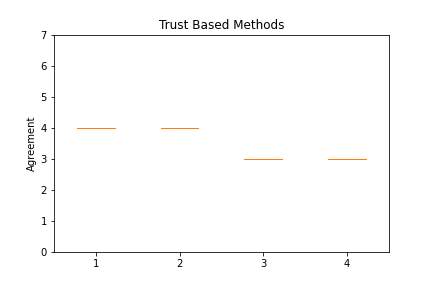
\includegraphics[width=0.5\textwidth]{main/Graphics/4ResultsandAnalysis/BoxPlot.png}
    \caption{A boxplot showing the four ratings for each question}
    \label{fig:Boxplot_Test}
\end{figure}

Overall comparison of all approaches with ranking if applicable. Produce a table for overall metric comparison. 

analysis: lead back to ui , vcompare with ui principles
% Carl

\section{Conclusion}
\label{sec:Conclusion}

Core results and their interpretation - which approach is evaluated as most promising and why, what are important pitfalls we observed. Refer to SoA for assessment and how our results fit in with that.

we evaluate that colouring and xy are among the most import factors for xai designers. what are the points they have to consider, what does a sw engineer need to take into account?

evaluation helps me to evaluate whether i can trust this, how do you do that?

\section{Future work}
\label{sec:FutureWork}
\section*{Acknowledgements}

We are grateful for the support of Mister Helpful for helping in shuffling. All Authors declare that there are no conflicts of interests. This work does not raise any ethical issues. This work was done in the context of EMPAIA Germany. Parts of this work have received funding from the Austrian Research Promotion Agency (FFG) under grant agreement No. 879881 (EMPAIA) and by the Austrian Science Fund (FWF), Project: P-32554 explainable Artificial Intelligence. 


\bibliography{references}

% \section*{About the Authors}

% \parpic{
\includegraphics[width=1in,clip,keepaspectratio]{bio-images/dummy.jpg}}
%\noindent {\bf Author Name} is the most famous author in her field. 
%She is particularly interested in X and Y, and also dabbles in Z.

% \bio{bio-images/evans.png}
% Theodore Evans received his M.Phys. degree in physics from the University of Manchester. He is a Ph.D. Candidate at the Distributed Artificial Intelligence Laboratory (DAI-Labor) of the Technisches Universität Berlin (TU-Berlin). He is currently supervised by Prof. Dr. Dr. hc Sahin Albayrak. His research interests lie in representation learning and cross-disciplinary approaches to explainable AI-assistance for digital pathology.
% \endbio

%\bio{bio-images/dummy.jpg}
%Max Mustermann is senior researcher at the awesome explainability Lab at the wonderful university of dreamland, and he is visiting researcher at the institute paradise in fantasy land. He received his Masters in computer science and her PhD in Computer Science from top university x. Erika is a member of the prestigious club wonder. 
%\endbio

% \bio{bio-images/holzinger.jpg}
% Andreas Holzinger is Visiting Professor for explainable AI at the University of Alberta, Canada since 2019 and head of the Human-Centered AI Lab at the Medical University Graz, Austria. He received his PhD in cognitive science from Graz University and his second PhD in computer science from Graz University of Technology. Andreas is ordinary member in the Academia Europaea, the European Academy of Sciences in the section Informatics, and full member of the European Lab for Learning and Intelligent Systems.
% \endbio

\end{document}


